\documentclass[11pt,a4paper]{article}
\usepackage[T1]{fontenc}
\usepackage[utf8]{inputenc}
\usepackage[spanish,es-noquoting]{babel}
\usepackage{amsmath}
\usepackage{booktabs}
\usepackage{graphicx}
\usepackage{siunitx}
\usepackage[margin=2.4cm]{geometry}
\usepackage[colorlinks=true,linkcolor=black,urlcolor=blue,citecolor=black]{hyperref}
\sisetup{output-exponent-marker=\text{e}}

\title{¿Se aparta la fricción de fondo calculada cuando el flujo deja de ser lento?\\
\large Barrido en $\delta$, etapa 1 --- caso \emph{forzado}, $\epsilon = 1.78$}
\author{Proyecto final --- capa delgada con superficie libre}
\date{16 de September de 2026}

\begin{document}
\maketitle

\section{Qué está en juego}

El trabajo afirma que el coeficiente de fricción de fondo se puede \emph{calcular} en vez
de ajustarlo: $\alpha = \pi^2\nu/4h^2$ para fondo no deslizante y tope free-slip. Esa
afirmación descansa en una clausura de un solo modo vertical, y la pregunta abierta
[P-01] es hasta dónde vale. El parámetro que la gobierna es
\begin{equation}
  \delta = \frac{U k h^2}{\nu} = \mathrm{Re}_h\,\epsilon , \qquad \epsilon = k h ,
\end{equation}
que compara la advección con la difusión viscosa vertical. En la celda medida $\delta$ va
de $\sim 20$ al arranque del registro a $\sim 1$ al final, así que la pregunta no es
académica.

Dos cosas quedaron sin resolver analíticamente. La estimación de la distorsión del perfil
vertical lleva un factor geométrico $O(1)$ que no se calculó, y el orden del sesgo sobre
$\alpha$ depende de la estructura horizontal del campo: para un único modo celular la
realimentación se anula hasta $O(\delta^2)$ por selección de números de onda, pero un
campo de banda ancha no tiene esa protección. Las dos se cierran midiendo.

\section{El método, y por qué así}

Se integra la ecuación de Navier--Stokes incompresible con el esquema de partición de
Fontana \emph{et al.}~\cite{fontana2020}, con fondo no deslizante y tope free-slip,
y se mide la tasa de decaimiento $\lambda$ de $\langle v^2\rangle$ sobre una ventana
tardía, entre 3.00 y 4.25 memorias modales $h^2/(2\pi^2\nu)$ desde el arranque:
la pregunta [P-02] es sobre la ventana del ajuste experimental, a más de cinco memorias
del corte, con el perfil vertical en balance cuasi-estacionario con el término no lineal
([D-42]). Además, sobre el campo escrito en el medio de esa ventana se mide directamente
$\alpha_\text{eff} = \nu\,\langle \partial_z u_h|_0 \cdot \bar U_h\rangle / (h\,\langle|\bar U_h|^2\rangle)$,
la fricción de fondo \emph{sin} clausura, que vale exactamente $\alpha$ para el perfil
$\sin(\pi z/2h)$; y el $k$ horizontal pesado por energía, que es el que entra en $\delta$.

\paragraph{El caso.} $\epsilon = kh = 1.78$ reproduce el régimen \emph{forzado} del
experimento ([D-41]): con el paso real de la red de imanes, el estado forzado y el arranque
del decaimiento están en $\epsilon = 1{,}78$, y la ventana del ajuste de $\alpha$
($t > 10$~s), con la energía ya migrada a $k \approx 60$--$130$~m$^{-1}$, en
$\epsilon \approx 0{,}35$--$0{,}8$. El modo dominante de la condición inicial es el diagonal,
$|k| = \sqrt2$ en unidades de código, así que $L_z = \epsilon/\sqrt2$.

\paragraph{La referencia lineal se mide, no se escribe.} El punto de comparación sale de
correr \emph{el mismo binario, la misma malla y la misma condición inicial} a amplitud
$u_0 = \num{1e-4}$, dos órdenes por debajo de la corrida más chica del barrido, donde
el término no lineal es despreciable por construcción. Así la referencia incluye
automáticamente el $k$ discreto de la malla, el sesgo del integrador y el filtro de
\emph{dealiasing}, y el cociente $\lambda/\lambda_\text{lin}$ es un número puro:
cualquier apartamiento es no linealidad y nada más. Escribir la fórmula analítica habría
mezclado el efecto buscado con los errores de discretización.

\paragraph{Dos resoluciones horizontales, y no es opcional.} El hallazgo [H-09] de este
mismo proyecto mostró que con el tope free-slip el término no lineal se desestabiliza sobre
mallas donde el canal aguanta: a amplitud alta y malla chica la energía \emph{crece} sin
forzado, que es imposible. Un apartamiento que no converge al refinar es numérico, no
físico. Por eso todo el barrido se corre a $16\times16$ y a $32\times32$.

\paragraph{Parámetros.} Caja $2\pi\times2\pi\times1.2567$, $\nu = \num{6.317e-02}$
(escalada con $L_z^2$ para que el tiempo de código sea el mismo múltiplo de $h^2/\nu$ en
los dos casos), $N_z = 64$ con $C_z = 25$ puntos de continuación, Runge--Kutta de
orden 2, $\Delta t = \num{5e-04}$ (un sexto del límite de estabilidad viscosa
explícita), 11905 pasos hasta $t = 5.952$, es decir 4.7 memorias
modales. Las amplitudes $u_0$ se eligieron para cubrir $\delta$ objetivo
0.3, 1, 3, 10, 20, 30 en la ventana; el $\delta$ de la tabla es el medido ahí.

\paragraph{El criterio, fijado antes de mirar los resultados.} Se declara que
\emph{hay} apartamiento si alguna corrida estable se aparta más que la barra de error del
$\alpha$ medido en el experimento, 7.3\,\%~[V-13], \emph{y} ese apartamiento
converge con la resolución (las dos mallas coinciden dentro de un tercio del efecto). Si
todas las corridas estables quedan dentro de esa barra, \emph{no hay}. Si hay apartamiento
pero no converge, el resultado es \emph{no concluyente}. El veredicto de la
sección~\ref{sec:res} lo produce el código, no el autor.

\section{Resultados}
\label{sec:res}

\begin{table}[h]
\centering
\begin{tabular}{lrrrrrr}
\toprule
& \multicolumn{6}{c}{$\delta$, $\lambda/\lambda_\text{lin}$ y $\alpha_\text{eff}/\alpha$ por malla}\\
\cmidrule(l){2-7}
$u_0$  & \multicolumn{3}{c}{$16\times16$} & \multicolumn{3}{c}{$32\times32$} \\ & $\delta$ & $\lambda/\lambda_\text{lin}$ & $\alpha_\text{eff}/\alpha$ & $\delta$ & $\lambda/\lambda_\text{lin}$ & $\alpha_\text{eff}/\alpha$ \\
\midrule
\num{4.44e-02} & 0.297 & 1.00018 & 1.0010 & 0.297 & 1.00018 & 1.0010 \\
\num{1.48e-01} & 0.983 & 1.00198 & 1.0040 & 0.983 & 1.00198 & 1.0040 \\
\num{4.44e-01} & 2.82 & 1.01432 & 1.0282 & 2.82 & 1.01432 & 1.0282 \\
\num{1.48e+00} & 7.26 & 1.00654 & 1.1548 & 7.26 & 1.00722 & 1.1547 \\
\num{2.96e+00} & 11.2 & 0.85968 & 1.1824 & 11.1 & 0.84311 & 1.1712 \\
\num{4.44e+00} & 14.4 & 0.81262 & 1.1869 & 14.4 & 0.72029 & 1.1206 \\
\bottomrule
\end{tabular}
\caption{Tasa de decaimiento medida, normalizada por la de la corrida lineal de
referencia de la misma malla, y $\alpha_\text{eff}/\alpha$ medido sobre el campo escrito
en el medio de la ventana. $\delta$ es el medido ahí, con el $k$ horizontal del propio
campo; dentro de la ventana cae un 25\,\%.}
\end{table}

\begin{figure}[h]
\centering
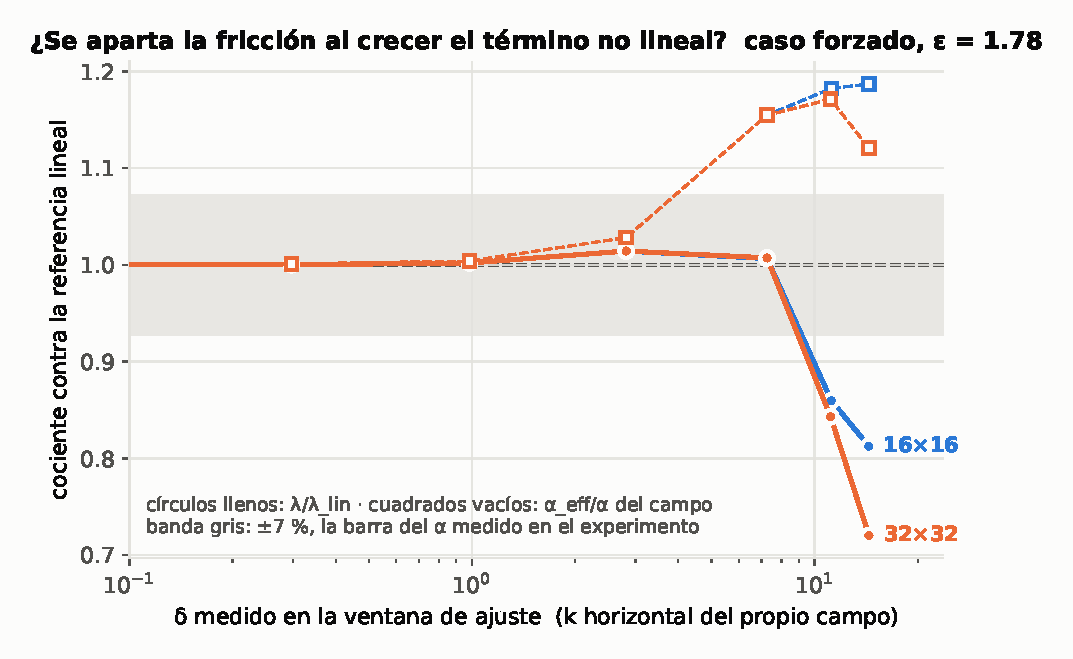
\includegraphics[width=\linewidth]{../salidas/figuras/f7_barrido_delta_forzado.pdf}
\caption{Cociente entre la tasa medida y la lineal, contra $\delta$, para las dos mallas.
La banda gris es la barra de error del $\alpha$ medido en el experimento. Las cruces
marcan corridas en las que la energía creció, o sea numéricamente inestables, que no se
usan.}
\end{figure}

\section{Veredicto}

\textbf{Hay apartamiento, y converge con la resolución.} El máximo es
27.97\,\%, por encima de la barra experimental (7.3\,\%), y las dos mallas
coinciden dentro de 9.23\,\%, de modo que no es un artefacto de resolución. La
clausura de un modo se rompe en el rango de $\delta$ cubierto, y la comparación
de~[V-13] tiene que corregirse por este efecto o restringirse a la cola del registro.

\section{Lo que esto no contesta}

La tasa $\lambda$ de $\langle v^2\rangle$ mezcla tres cosas: la fricción de fondo, la
disipación viscosa horizontal y la transferencia no lineal entre escalas. Por eso se mide
además, sobre el campo, $\alpha_\text{eff}$ de la ecuación de la sección~2, que aísla el
corte en el fondo sin ninguna clausura. Que las dos medidas se muevan juntas dice que el
apartamiento está en la fricción y no sólo en la redistribución de energía entre escalas.

Salvedades que quedan: la condición inicial es un campo de dos modos horizontales con el
perfil vertical fundamental, no un campo de banda ancha como el del experimento, y la
realimentación no lineal sobre la tasa depende de esa estructura; la simulación decae
libremente, mientras que la meseta del experimento es un estado forzado; y $\delta$ se
calibra con el $k$ horizontal pesado por energía del propio campo en el medio de la
ventana, y dentro de ella $\delta$ cae un 25\,\%, así que cada punto representa un rango
y no un valor. El $\langle v^2\rangle$ de \texttt{balance.txt} está promediado sobre el
dominio físico y coincide con el del campo escrito; el $\langle\omega^2\rangle$ del mismo
archivo no reproduce el rotor del campo y no se usa ([H-17]).

\begin{thebibliography}{9}
\bibitem{fontana2020} M.~Fontana, O.~P.~Bruno, P.~D.~Mininni y P.~Dmitruk,
\emph{Fourier continuation method for incompressible fluids with boundaries},
Comput. Phys. Commun. \textbf{256}, 107482 (2020).
\href{https://doi.org/10.1016/j.cpc.2020.107482}{doi:10.1016/j.cpc.2020.107482}.
Leído en el original en sus secciones 2, 4.1, 4.2 y 4.4.
\bibitem{orszag1986} S.~A.~Orszag, M.~Israeli y M.~O.~Deville,
\emph{Boundary conditions for incompressible flows},
J. Sci. Comput. \textbf{1}, 75 (1986).
\href{https://doi.org/10.1007/BF01061454}{doi:10.1007/BF01061454}.
Origen de las condiciones de contorno sobre $v^*$ y sobre $p$ que usa el solver.
Localizado y verificado en Crossref; \emph{no} leído en el original, es de acceso cerrado.
\bibitem{kio1991} G.~E.~Karniadakis, M.~Israeli y S.~A.~Orszag,
\emph{High-order splitting methods for the incompressible Navier--Stokes equations},
J. Comput. Phys. \textbf{97}, 414 (1991).
\href{https://doi.org/10.1016/0021-9991(91)90007-8}{doi:10.1016/0021-9991(91)90007-8}.
Su sección 2.3 se aplicó al esquema de este solver en~[V-15].
\end{thebibliography}

\end{document}
